\documentclass[landscape,paperwidth=43truein,paperheight=33.1truein,fontscale=0.3]{baposter}
\usepackage{graphics}
\usepackage{color}
\usepackage{multicol}
\usepackage{amsmath}
\usepackage{amssymb, wasysym}
\usepackage{lipsum}
\usepackage{graphicx}
\usepackage{enumitem}

\pdfcompresslevel=1

\begin{document}
\definecolor{myfavoritecolor}{rgb}{0.0 2.55 0}

%:Background image
\background{
      \begin{tikzpicture}[remember picture,overlay]%
      \draw (current page.center)+(-0em,-10em) node[anchor=center]
      {\includegraphics[width=1.2\textwidth]{images/teal_sun.png}};
      \end{tikzpicture}%
      }

\begin{poster}
{%Keyword=value pairs
  % Color style
background = user,
 bgColorOne=white,
  bgColorTwo=red,
  borderColor=black,
  headerColorOne=black,
  headerColorTwo=gray,
  headerFontColor=white,
  boxColorOne=white,
  boxColorTwo=myfavoritecolor,
  % Format of textbox
  textborder=roundedleft,
  % Format of text header
  eyecatcher=true,
  headerborder=closed,
  headerheight=0.15\textheight,
  headershape=roundedright,
  headershade=shadelr,
  boxshade=plain,
  headerfont=\Large\textrm,
}
{%Eyecatcher
   \resizebox{!}{.15\textheight}{
\includegraphics{images/sselpatch_transbg.png}}
}
{%Poster Title
   {\color{red}A Database System for Storing Satellite Data Requests}
}
{%Author
  \color{red} \textbf{Nevin Leh \\
   \textit{Physics Department, Montana State University, Bozeman, MT 59717}\\
   nevinleh@gmail.com}\\
}
{%Logo
   \resizebox{!}{.15\textheight}{
\includegraphics{images/msgc_2009_transbg.png}}
}

%%%%%%%%%%%%%%%%%%%%%%%%%%%%%%%%%%%%
%         Zeroth Column            %
%%%%%%%%%%%%%%%%%%%%%%%%%%%%%%%%%%%%

\headerbox{Abstract}{name=abstract,column=0}{
 The process of creating a database to process and manage data requests for the FIREBIRD-II (Focused Investigations of Relativistic Electron Burst Intensity, Range, and Dynamics) satellites has been underway for some time. The structure of such a database relies on the way data is stored and down linked. There have been several iterations of this database as new tools and information have become available and the current iteration contains several new features and bug fixes. The newest version is still under development and still needs some features such as control scripts to be used as a fully functional database system. 
  \vspace{0.33cm}
}

\headerbox{Design Challenges}{name=launch,column=1}{
\begin{tabular}{ll}
 \begin{minipage}{0.10\columnwidth}
      \resizebox{\columnwidth}{!}{\includegraphics{images/MOSESinFlight.png}}
   \end{minipage} &
   \begin{minipage}{0.80\columnwidth}
      \textit{MOSES} was 
      first launched on February 8, 2006 on a NASA sounding rocket. The next launch will include updated optics and electronics and is scheduled for summer 2015.
   \end{minipage} 
  
\end{tabular}
}

\headerbox{Design Challenges}{name=challenges,column=2}{
	The sounding rocket trajectory only provides approximately 5 minutes of data for the instrument to capture. To acquire data in real time and minimize risk to the experiment, the flight software must be efficient and use minimal resources. \vspace{.21cm}
}

\headerbox{Data Interface}{name=interface,column=1,span=2, below=launch}{

\begin{tabular}{ll}
  \begin{minipage}{0.50\columnwidth}
The new flight computer is designed as a drop-in replacement for the old flight computer, so it must interface with the instrument in the same manner. The primary means of starting and stopping the experiment are predefined \textbf{Timers}. Science data is acquired from the \textbf{ROE} using the \textbf{FPGA}. It is then transferred to the \textbf{VDX} using DMA and written to disk. For redundancy, the data is transmitted to earth using the \textbf{Synclink USB} interface and a 10 Mbit/s link.

  \end{minipage}&
  \begin{minipage}{0.45\columnwidth}
      \resizebox{\columnwidth}{!}{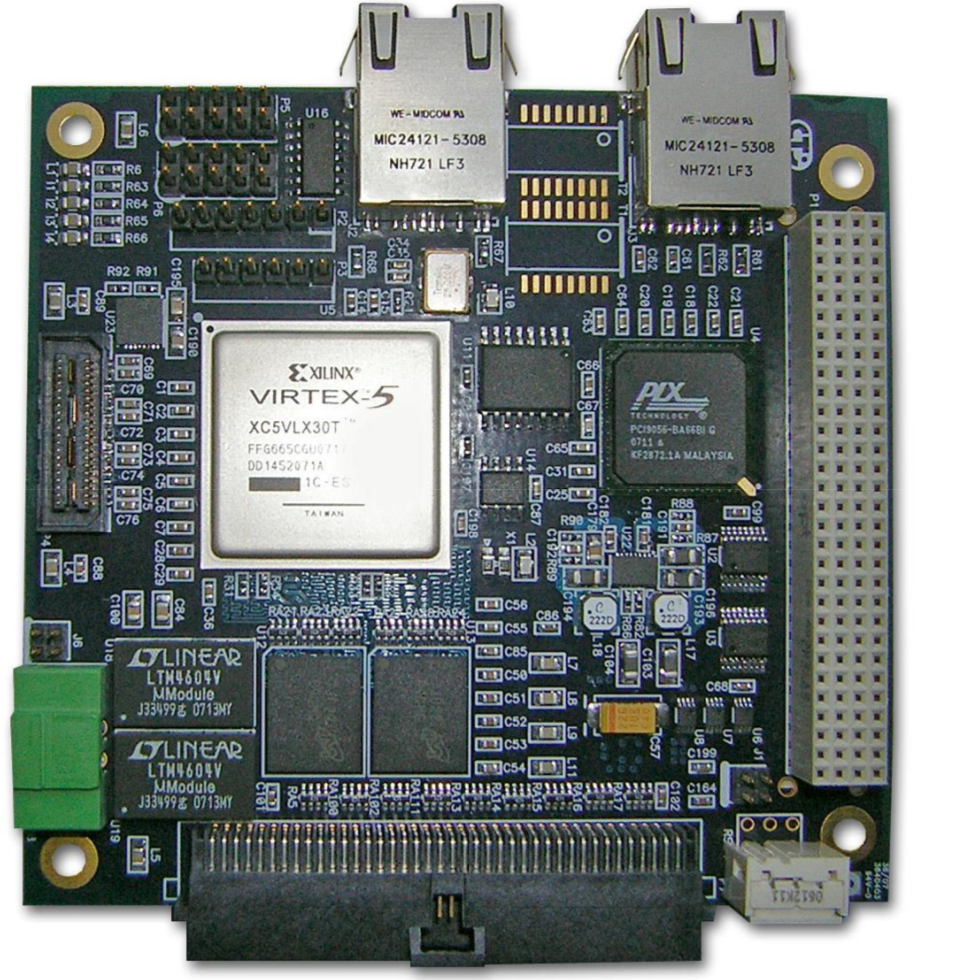
\includegraphics{images/fpga.png}}
      \footnotesize{Block diagram of major hardware components managed by flight software}  
\end{minipage}  
\end{tabular}


}
\headerbox{Hardware Solutions}{name=hardware,column=3}{
The VDX104+ running a Ubuntu GNU/Linux operating system is the flight computer for the instrument. It provides ethernet and RS-232 serial ports for communication, and PCI-104 bus for interfacing with the FPGA. The flight software designed by our team runs on this device.

\begin{tabular}{ll}
	\begin{minipage}{0.46\columnwidth}
  		\resizebox{\columnwidth}{!}{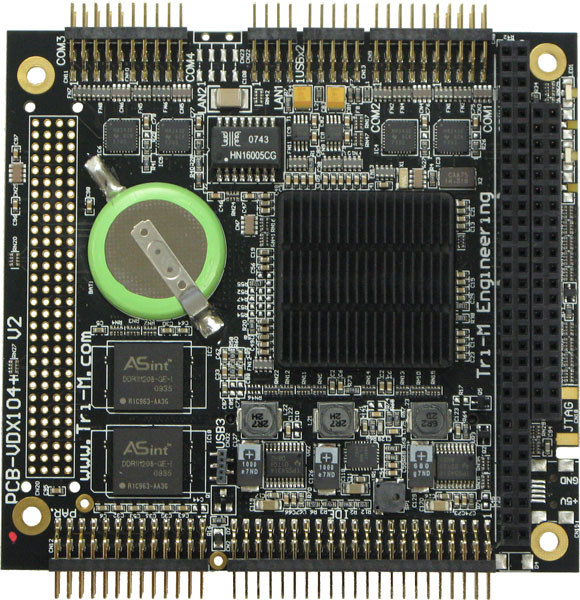
\includegraphics{images/vdx104}}  \\
  		\footnotesize{VDX104 flight computer}
	\end{minipage}&

  \begin{minipage}{0.46\columnwidth}
		\resizebox{\columnwidth}{!}{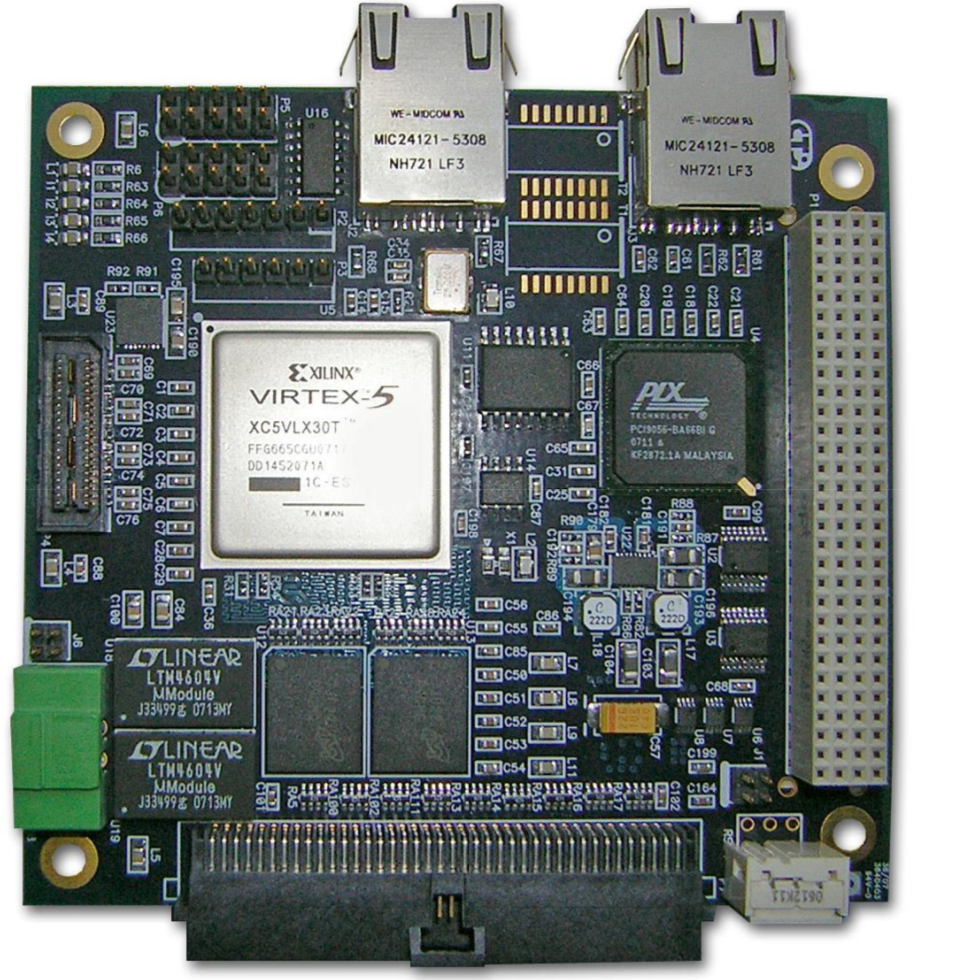
\includegraphics{images/fpga}} \\
		\footnotesize{ Virtex5 FPGA}
  \end{minipage}
\end{tabular} \\ \\
The Virtex5 FPGA captures the 32 Mbit/s parallel data produced by the experiment and various GPIO. It then transfers the data through DMA to the flight computer for processing.

}

\headerbox{Software Architecture}{name=arch,column=0,span=3, below=interface}{
\begin{tabular}{ll}
	\begin{minipage}{0.85\columnwidth}
      \resizebox{\columnwidth}{!}{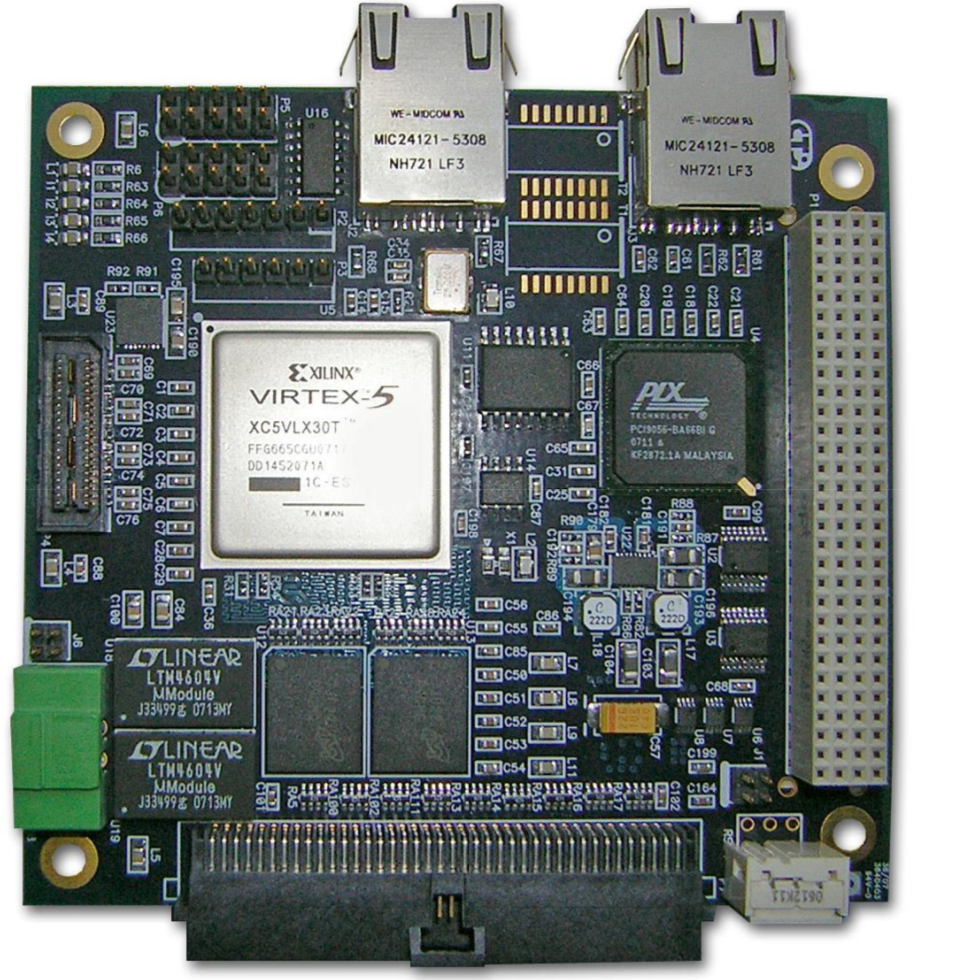
\includegraphics{images/fpga.png}}
      \footnotesize{Diagram of major software modules}  
	\end{minipage}&

  \begin{minipage}{0.10\columnwidth}
  	\raggedright
     The flight software relies on a threaded architecture to reliably respond to a variety of inputs, all while the processor is actively capturing data. Several thread-synchronization techniques have been utilized, including mutex-protected queues, Linux Signals, and semaphores. 

  \end{minipage}
    
\end{tabular}
}

\headerbox{Glossary}{name=gloss,column=3,below=hardware}{ 

%\begin{itemize} \itemsep1pt \parskip0pt \parsep0pt \itemindent=-0.5cm
\begin{itemize}[leftmargin=*, noitemsep]
\item \textbf{EUV:} Extreme Ultraviolet electromagnetic radiation.
\item \textbf{VDX:} Model name of flight computer board.
\item \textbf{FPGA:} Field-Programmable Gate Array. 
\item \textbf{ROE:} Read-Out Electronics. Hardware that captures science data from cameras.
\item \textbf{DMA:} Direct Memory Access. Protocol for copying data without involving the computer's processor.
\item \textbf{HLP:} Housekeeping Link Protocol. Packets transmitted from the ground that can control the instrument.
\end{itemize}
}


\headerbox{Acknowledgment}{name=ack,column=3,below=gloss}{ \footnotesize

\begin{minipage}{\columnwidth}
This work is supported by the NASA Sounding Rocket Program, Grant NNX14AK71G.
 
\end{minipage}
\normalsize
}


\headerbox{References}{name=refs,column=3,below=ack,above=bottom}{\footnotesize
\begin{minipage}{\columnwidth}
[0] Fox, Kankelborg and Thomas, 2010 \textit{Astrophys.J.}, 719:1132-1143

[1] Background image courtesy of the NASA Solar Dynamics Observatory
 
\end{minipage}
\normalsize}

\end{poster}

\end{document}